\documentclass[a4paper,12pt]{report}

\usepackage[francais]{babel}
\usepackage[T1]{fontenc}  
\usepackage[utf8]{inputenc}  
\usepackage{lmodern}  
\usepackage{color}  
\usepackage{graphicx}  
\usepackage{appendix}

\usepackage[
backend=biber,
style=alphabetic,
sorting=ynt
]{biblatex}




\title{Visualisation de matchs de football robotique}
\author{ 
\textit{Lucie CHASAN}\\
\textit{Florian ESCURE}\\
\textit{Lucie MATHÉ}\\
\textit{Eliott MONTERO}\\
} 
\date{9 avril 2019}

\begin{document}

\begin{figure}[!b]  
\begin{center}  

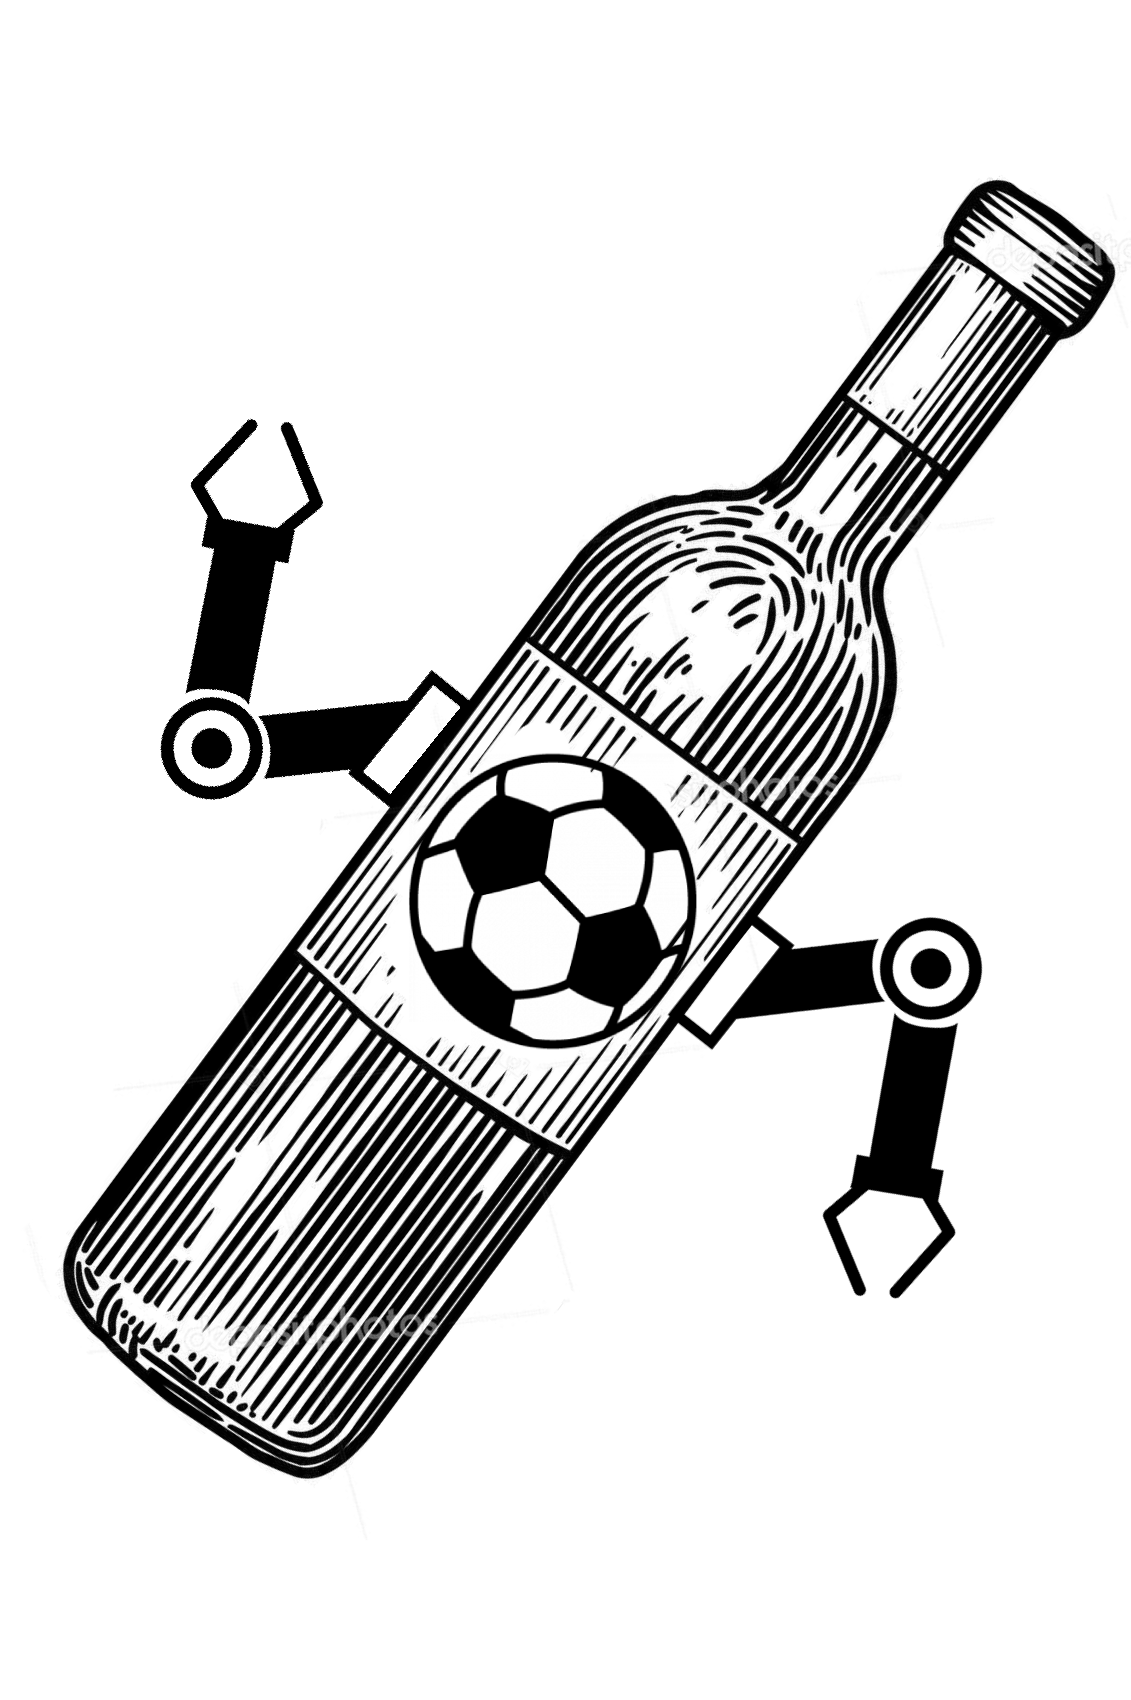
\includegraphics[scale=1]{vin.png}  
\end{center}  
\end{figure}  

\maketitle

\newpage
\chapter{Introduction}
A REFAIRE+schéma audit


La RoboCup est une compétition internationale où des robots autonomes s'affrontent dans des matchs de football. Afin d'améliorer la présentation des matchs aux spectateurs, il serait intéressant de proposer un outil permettant d'incruster dans un flux vidéo des informations sur l'état du jeu perçu par les robots.
\\

En plus de son utilisation lors des matchs, un tel outil permettrait de revoir des matchs en choisissant de manière dynamique des incrustations différentes, correspondant à la perception d'un robot, d'une équipe ou de données expertes.  
\\

L’incrustation des informations nécessitera d'écrire du code permettant de projeter des positions et des formes géométriques élémentaires sur le flux vidéo. 



\newpage



\chapter{Besoins}
 reprendre  cahier des besoins + différence par rapport à ce qu'on a fait
 
\section{Fonctionnels}


\section{Besoins non fonctionnels}

\chapter{Architecture du projet}

   
\section{Code fourni par le client}

Le code fourni par le client se compose de deux packages. 
Le premier package hl\_communication contient les classes nécessaire à la lecture des messages des robots. Les principales fonctions que l'on utilise de ce package sont contenues dans la classe MessageMonitoring.
\\

C'est grâce à un objet MessageMonitoring que nous allons pouvoir récupérer le message que le robots nous envoie pour chaque temps donné. 
Également, c'est grâce à hl\_communication que nous pouvons lire les . Proto et donc lire l'intérieur des messages.
\\

Le second package est hl\_monitoring. Il permet de lire la vidéo et d'adapter les données à la caméra.
Nous avons donc d'une part le MonitoringManager qui va récupérer l'image à un temps donné de la vidéo, et d'autre part des fonctions telles que fieldToImg qui vont nous permettre de transformer des positions du plan à l'image en fonction des paramètres de la caméra.
\\

Nous avons également une fonction permettant d'afficher les lignes du terrain et nous montrant le bon fonctionnement du monitoringmanager sur la vidéo.
\\

Le package hl\_monitoring contient également basic\_monitoring un exécutable permettant de tester tout ce qui nous a été fourni par le client. C'est dans ce fichier que nous avions fait nos premiers tests d'affichage avant d'en recréer un nous-même.

\section{Implémentation de la V1}

Lors de notre rendu de la V1 en début d'année, notre architecture n'était pas adaptée au projet.



   
\chapter{Fonctionnalité implémentées}

\section{Le traitement}

Pour l'ajout de certaines annotations comme la trace, nous avons souhaité utiliser la transparence. Ainsi, les anciennes positions deviennent graduellement transparentes, jusqu'à disparaître. Ceci permet une meilleure visibilité des déplacements. Malheureusement, les fonctions de dessin d'openCV ne gèrent pas la transparence. OpenCV gère bien les images avec transparence, les fonctions de dessin acceptent des couleurs avec transparence, mais lors du dessin, elles ignorent cette valeur et dessinent en pleine opacité. 
\\

Nous avons pensé à deux moyens de contourner ce problème : 
\begin{itemize}
    \item Coder des fonctions de dessin similaires à celles d'openCV mais gérant la transparence.
    \item Utiliser la fonction openCV combinant deux images en modifiant leur opacité.
\end{itemize}
\vspace{10pt}

C'est la deuxième option qui a été retenue. Pour afficher la trace, nous créons donc une petite image contenant le point de position, que nous incrustons avec une opacité variable sur l'image du match. Le nombre de positions à afficher peut être modifié, l'opacité diminue avec l'âge de la position. 




\section{L'interface}
Nous ajoutons des annotations sur une vidéo de match. Cependant, étant donné le grand nombre d'informations, l'image peut se trouver saturée et devenir illisible. Notre interface doit résoudre ce problème en proposant des options d'affichage qui conviennent à différents usages.
\\


Dans un premier temps, il a fallu choisir une API pour créer l'interface de notre programme. Nous en cherchions une plutôt facile à prendre en main, en c++, et qui propose suffisamment d'options pour créer une interface complète. 
\\

Nous avons d'abord pensé à openCV, que nous utilisons déjà abondamment pour les annotations. La prise en main est assez rapide mais les options sont trop peu nombreuses. Les interfaces en openCV se limitent principalement à afficher des images, sans trop de fioritures. 
\\

GTK et FLTK ont été rapidement considérés, mais la prise en main semblait trop compliquée et aurait pris trop de temps. 
\\

Nous avons donc choisit QT dans sa version 5.9, qui est très bien documenté, facile à prendre en main et présente un très large éventail d'options pour créer une interface riche et complète.
\\

Au début du projet, nous avons rencontré des difficultés pour faire communiquer l'interface et les fonctions d'annotation. Après la refonte de l'architecture du projet, la liaison entre les modules interfaces et traitement était grandement simplifiée, et nous avons pu lire une vidéo dans notre fenêtre QT. 
\\

Nous avons ensuite pu ajouter des options pour choisir les annotations à afficher, modifiables pendant la lecture de la vidéo. 
\\

Et un slider.
\\

Asseyons nous 5 minutes et parlons de la merveille qu'est ce slider. 
\\

Déjà il ressemble à un slider, il s'appelle slider, il occupe une bonne partie de la fenêtre comme un slider.
MAIS ce n'est pas un slider, non non non.
Parce que quand on clique sur le slider, la vidéo bouge. Elle bouge vite, très vite. en vérité elle avance. de 2 secondes à chaque mouvement du slider. C'est donc le premier slider à avance rapide. Pour simplifier l'utilisation et éviter les erreurs, nous avons choisi de bloquer le retour en arrière. Le saut de 2s nous a semblé pertinent : ni trop long ni trop court. 
\\

Nous essaierons de le faire fonctionner ce WE comme un vrai slider pour choisir le moment de la vidéo.
\\

De chaque coté de la vidéo, nous affichons des informations sur le déroulement du match, les robots et les équipes.




\subsection{Interface Débug}
Cette interface est celle qui propose le plus d'options. L'utilisateur choisit quelles annotations seront affichées et pour quel(s) robot(s). 
\\

Pour alléger l'interface, la sélection des éléments à afficher se fait dans une fenêtre surgissante. L'utilisateur coche les annotations qui l'intéressent, valide, puis choisit les robots sur la fenêtre principale. Le changement prend effet dès l'image suivante.  

\newpage
\chapter{Tests effectués}

\section{Le traitement}

\subsection{Tests sur l'utilisation du Json}

Tous les réglages des annotations s'effectuent dans le fichier annotation\_settings.json. Nous avons donc testés les différents problèmes que nous pouvons rencontrer dans la lecture de ce fichier JSon.
\\

\begin{itemize}
    \item \textbf{Il manque un item dans le fichier} : Pour tous les éléments utilisés nous utilisons une fonction \textit{CheckMember} qui va vérifier qu'il ne manque pas d'informations dans le fichier Json. 
    
    Il faut noter que même si une annotation n'est pas utilisée, nous vérifions que tous ses items sont là. En effet, grâce à l'interface nous pouvons changer les annotations sans relancer notre exécutable. Il est donc important de vérifier que tous les objets du Json sont présent dès le début afin de pouvoir les utiliser si besoin en changeant les annotations.
    \item \textbf{Un item a été ajouté en trop} : Les éléments présents dans le fichier annotation\_settings.json mais non utilisés dans nos fonctions ne gênent en aucun cas l'ajout des annotations dans la vidéo. Ils sont justes ignorés.
    \item \textbf{Un item est présent deux fois dans le fichier} : Nous avons testé ce cas là en dupliquant des éléments du Json. Dans ce cas là, la dernière itération de l'élémént sera celle prise en compte.
\end{itemize}

\subsection{Tests sur la lecture des logs}

Nous avons essayé de rendre notre programme le plus optimisé possible dans la lecture des logs. Nous avons pour cela identifié un problème majeur que l'on peut trouver en match : l'interruption de l'envoi des messages par les robots. Les tests sur l'interruptions des logs s'effectuent dans le fichier test.cpp, dont l'exécutable est tools/test\_pos.

Pour cela nous avons eu besoin d'identifier les dépendances entre les différentes annotation.

\begin{itemize}
    \item \textbf{La Position } : rien.
    \item \textbf{La Direction }: Nécessite la Position.
    \item \textbf{La Balle }: Nécessite la Direction et la Position.
    \item \textbf{La Trace }: Nécessite au moins une Position.
    \item \textbf{La Position souhaitée } : Nécessite la Position actuelle pour avoir le trajet à effectuer par le robot, sinon rien.
\end{itemize}

Nous voyons ici que la position du robot est essentielle pour presque toutes les annotations. Si l'on lance le fichier de test d'annotations avec la vidéo du répertoire 2vs1, nous remarquons donc que le robot 2 de l'équipe 9 n'affiche aucune annotation.

Enfin dans ce fichier de test nous interrompons les différentes annotations. 



\section{L'interface}


\chapter{Conclusion}

conclu+suites du projet

\newpage

\printbibliography

\newpage


\end{document}
